\documentclass{beamer}
\usetheme{Boadilla}
\usepackage{tikz}
\title{Presentation EE1390}
\author{Sumanth, Sravan}
\date{\today}
\begin{document}
\maketitle
\begin{frame}{Question}
Verify if the circles $C_1 : x^2+y^2=1$  and  $C_2 : (x+7)^2+(y-1)^2=49$ are orthogonal.
\end{frame}

\begin{frame}{Solution}
$C_1 : x^2+y^2=1$ \hspace{1cm}  $C_2 : (x+7)^2+(y-1)^2=49$\\
\vspace{5mm}
General form of a circle = $x^T V x + 2u^T x + F = 0$\\
\vspace{3mm}
For circle C_1 :
$$V_1$$=\begin{bmatrix}
    1 &0\\
    0 &1
    \end{bmatrix}
\hspace{3mm}
$$u_1$$=\begin{bmatrix}
    0\\
    0
    \end{bmatrix}
\hspace{3mm}
F_1=-1\\
\vspace{4mm}
For circle C_2 :
$$V_2$$=\begin{bmatrix}
    1 &0\\
    0 &1
    \end{bmatrix}
\hspace{3mm}
$$u_2$$=\begin{bmatrix}
    1\\
    -1
    \end{bmatrix}
\hspace{3mm}
$F_2=1$
\end{frame}
\begin{frame}{Matrix transformation of the question}
    Verify if the circles $C_1$: $x^T\begin{bmatrix}
    1 &0\\
    0 &1
    \end{bmatrix}x + 2\begin{bmatrix}
    0 &0
    \end{bmatrix}x -1 = 0$
    and\\ $C_2$ : $x^T\begin{bmatrix}
    1 &0\\
    0 &1
    \end{bmatrix}x + 2\begin{bmatrix}
    1 &-1
    \end{bmatrix}x + 1 = 0$ are orthogonal.
\hspace{3mm}
\end{frame}
\begin{frame}
    Tangent to any circle at Point P is $(P^T V +u^T)x + P^T u +F = 0$\\
    \vspace{3mm}
    Let P be the point of intersection of $C_1$ and $C_2$\\
    \vspace{3mm}
    Tangent to $C_1$ at P is $(P^T V_1 +u_1^T)x + P^T u +F_1 = 0$\\
    \vspace{3mm}
    $T1 : (P^T +u_1^T)x + P^T u_1 -1 = 0 $\\
    \vspace{3mm}
    \vspace{3mm}
    \vspace{3mm}
    Tangent to $C_2$ at P is $(P^T V_2 +u_2^T)x + P^T u_2 +F_2 = 0$\\
    \vspace{3mm}
    $T2 : (P^T +u_2^T)x + P^T u_2 + 1 = 0 $
\end{frame}
\begin{frame}
    For orthogonality these tangents have to be perpendicular.\\
    \vspace{3mm}
    Direction vector $T_1$ is $D_1$ : $P^T +u_1^T$\\
    \vspace{3mm}
    Direction vector $T_2$ is $D_2$ : $P^T +u_2^T$\\
    \vspace{3mm}
    Orthogonality condition : $D_1D_2^T$=0\\
    \vspace{3mm}
    $(P^T + u_1^T)(P + u_2) = 0$\\
    \vspace{3mm}
    $P^TP + P^Tu_2 + u_1^TP + u_1^Tu_2 = 0$
\end{frame}
\begin{frame}{Result}
    One point of intersection of $C_1$ and $C_2$ is P = \begin{bmatrix}
    0\\
    1
    \end{bmatrix}\\
    \vspace{3mm}
    On substituting in previous equation we get\\
    \vspace{3mm}
    \vspace{3mm}
    \begin{bmatrix}
    0 &1
    \end{bmatrix}\begin{bmatrix}
    0 \\1
    \end{bmatrix} +\begin{bmatrix}
    0 &1
    \end{bmatrix}\begin{bmatrix}
    1 \\-1
    \end{bmatrix} + \begin{bmatrix}
    0 &0
    \end{bmatrix}\begin{bmatrix}
    0 \\1
    \end{bmatrix}+\begin{bmatrix}
    0 &0
    \end{bmatrix}\begin{bmatrix}
    1 \\-1
    \end{bmatrix} = 0\\
    \vspace{3mm}
    \vspace{3mm}
    As we proved for one point of intersection the the tangents will also be perpendicular at the other point of intersection.\\
    \vspace{3mm}
    \vspace{3mm}
    Therefore the circles are orthogonal.
\end{frame}
\begin{frame}{Tangents}
    $T1 : (P^T +u_1^T)x + P^T u_1 -1 = 0 $\\
    (\begin{bmatrix}
    0 &1
    \end{bmatrix} + \begin{bmatrix}
    0 &0
    \end{bmatrix})x + \begin{bmatrix}
    0 &1
    \end{bmatrix}\begin{bmatrix}
    0 \\
    0
    \end{bmatrix} - 1 = 0\\
    = \begin{bmatrix}
    0 &1
    \end{bmatrix}x = 1\\
    \vspace{2mm}
    Which implies $T_1$ : Line y=1\\
    \vspace{3mm}
    $T2 : (P^T +u_2^T)x + P^T u_2 + 1 = 0 $\\
    (\begin{bmatrix}
    0 &1
    \end{bmatrix} + \begin{bmatrix}
    1 &-1
    \end{bmatrix})x + \begin{bmatrix}
    0 &1
    \end{bmatrix}\begin{bmatrix}
    1 \\
    -1
    \end{bmatrix} + 1 = 0\\
    = \begin{bmatrix}
    1 &0
    \end{bmatrix}x = 0\\
    \vspace{2mm}
    Which implies $T_2$ : y-axis\\
\end{frame}
\begin{frame}{Figure}
    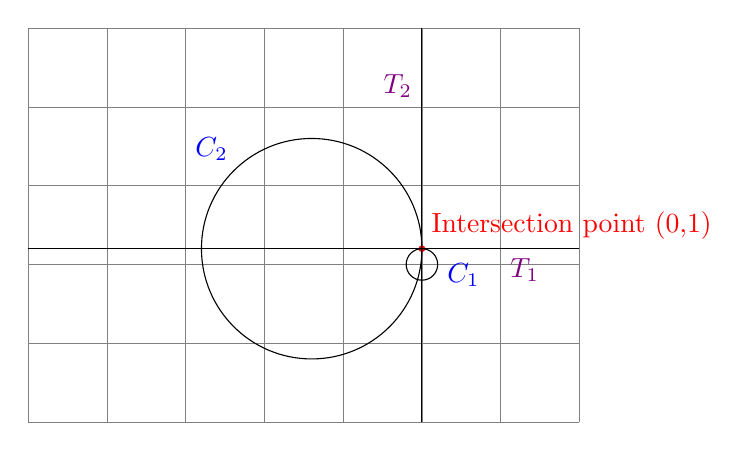
\begin{tikzpicture}
    \draw[step=1cm,gray,very thin] (-5,-2) grid (2,3);
    %\draw (-5,0) -- (2,0);
    \filldraw[red] (0,0.2) circle (1pt) node[anchor=south west] {Intersection point (0,1)};
    \filldraw[blue] (-3,1.2) node[anchor=south west] {$C_2$};
    \filldraw[blue] (0.2,-0.4) node[anchor=south west] {$C_1$};
    \filldraw[violet] (0,2) node[anchor=south east] {$T_2$};
    \filldraw[violet] (1,0.2) node[anchor=north west] {$T_1$};
    \draw (0,-2) -- (0,3);
    \draw (-5,0.2) -- (2,0.2);
    \draw (0,0) circle (2mm);
    \draw (-1.4,0.2) circle (14mm);
    \end{tikzpicture}
\end{frame}
\end{document}



